\chapter{Conclusions}

\section{Further work} \label{Further work}

\subsection{Hardware}
\paragraph{The Xaviers} could be switched out with computers using x86 processor for limiting sources of error. 

\paragraph{}

\subsection{Improving platooning algorithms}
\paragraph{Time Delay} algorithm is working and can be improved with more information into the "subpub" node. The node can subscribe to odometry of Husky and TB3, and use this information to calculate the offset of where the TB3 is and where it should be. When Husky drives with Nav2 the topic \topic{/path} can be used for improving where the averness of where teh TB3 should be. Potentially LiDAR data can also be used, and the algorithm could be improved forever. Continuing improving on Time Delay feels like building a bad of Nav2. Therefor the author of this thesis believe using Nav2 API is the best way to achieve autonomous platooning with ROS2. 

\paragraph{Nav2 API} was initiated but remained unfinished due to time constraints. This method is based on the Nav2 API and the fact that the TB3 and the Husky have been setup with the ability to drive autonomously independently. For better understanding here is a list of some Nav2 API commands.

\begin{table}[H]
    \centering
    \begin{tabular}{c|c}
        Command             & Description \\ \hline
        setInitialPose()    & Setting initial pose of a robot \\
        goToPose()          & Publishes a Nav2 Goal \\
        goThroughPoses()    & Publishes a list of Nav2 Goals \\
        getPath()           & Receives the complete ongoing path \\
        changeMap()         & Changes current map to chosen one \\
        getFeedback() & Info about the robot running Nav2 like Time stamp, frame\_id and pose\\
    \end{tabular}
    \caption{Some Nav2 API commands \cite{rosnavAPI}}
    \label{tab:Nav2API}
\end{table}

The idea was both husky and TurtleBot3 run Nav2, a node receives "getFeedback()" from Husky and sends "goToPose()" x distance behind the Husky to the TB3. This task was started on but not finished here is a list with status of the milestones \ref{tab:MilestonesNav2API}.
%move to future work
\begin{table}[H]
    \centering
    \begin{tabular}{c|c}
        Task                                                        & Status   \\ \hline
        Husky driving autonomously with Nav2                        & Complete \\
        TB3 driving autonomously with Nav2                          & Complete \\
        Control Nav2 with API from python                           & Complete \\
        Husky with namespace                                        & Not complete \\
        TB3 with namespace                                          & Complete \\
        Running Nav2 on Husky with namespace                        & Not complete \\
        Running Nav2 on TB3 with namespace                          & Not complete \\
        Running Husky and TB3 on same network with independent Nav2 & Not complete\\
        Node receiving position from Husky and sending goal to TB3  & Not complete \\
    \end{tabular}
    \caption{Milestones of Nav2 API}
    \label{tab:MilestonesNav2API}
\end{table}

The main challenge is running two robots with Nav2 simultaneously on the same network. It may be that both robots need two be able to run Nav2 with namespace, but probably just one. Launching two robots may be possible with using the standard launch files from Nav2. It is also possible a custom launch file need to be build using Nav2 nodes like this video \cite{MultiRobotNav2}.
   

\paragraph{AprilTags/ArUco} where researched but not tested. AprilTags and ArUco markers is a system where a camera can get a tf from viewing the tag seen in Figure \ref{fig:apriltags} and demonstrated in Figure \ref{fig:apriltag_principal}. When a tf between TB3 and Husky is acquired this can be used to make a platooning system or improve on an existing one. 

\begin{figure}[H]
  \centering
  \begin{minipage}[b]{0.4\textwidth}
    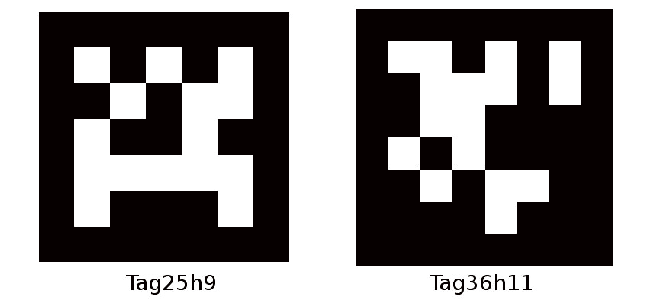
\includegraphics[width=\textwidth]{Figures/images/apriltags.png}
    \caption{Example of two AprilTags}
    \label{fig:apriltags}
  \end{minipage}
  \hfill
  \begin{minipage}[b]{0.4\textwidth}
    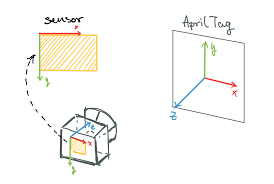
\includegraphics[width=\textwidth]{Figures/images/apriltag_prinsipal.png}
    \caption{Drawing showing the principal of AprilTags}
    \label{fig:apriltag_principal}
  \end{minipage}
\end{figure}
